\documentclass[11pt,a4paper]{article}

\usepackage[utf8]{inputenc}
\usepackage[T5,T1]{fontenc}
\usepackage[vietnamese]{babel}
\usepackage{geometry}
\geometry{
    top=20mm,
    bottom=20mm,
    left=22mm,
    right=22mm,
    headheight=15pt,
    headsep=12pt
}

\usepackage{graphicx}
\usepackage{xcolor}
\usepackage{listings}
\usepackage{hyperref}
\usepackage{fancyhdr}
\usepackage{tabularx}
\usepackage{booktabs}
\usepackage{tikz}
\usepackage{amsmath}
\usepackage{tcolorbox}
\usepackage{caption}

% Thiết lập liên kết URL
\hypersetup{
    colorlinks=true,
    linkcolor=blue!80!black,
    urlcolor=blue!80!black
}

% Định nghĩa Logo BK bằng TikZ để biên dịch độc lập không cần file ảnh ngoài
\newcommand{\bklogo}{%
    \begin{tikzpicture}[baseline=(bk.base)]
        \node[draw=blue!80!black, fill=blue!80!black, text=white, font=\bfseries\sffamily\scriptsize, rounded corners=1.5pt, inner sep=2.5pt] (bk) {BK};
    \end{tikzpicture}%
}

% Cấu hình Header & Footer giống file đề gốc của thầy
\pagestyle{fancy}
\fancyhf{}
\lhead{\includegraphics[height=20pt,keepaspectratio]{"images/Logo BK.png"}\hspace{8pt}\raisebox{4pt}{\small\sffamily Faculty of Computer Science and Engineering -- HCMC University of Technology}}
\rhead{\raisebox{4pt}{\small\sffamily Computer Networks (CO3093)}}
\cfoot{\thepage}
\renewcommand{\headrulewidth}{0.5pt}

% Cấu hình listings hiển thị code
\lstset{
    language=Java,
    basicstyle=\fontsize{9}{11}\ttfamily,
    keywordstyle=\color{blue}\bfseries,
    stringstyle=\color{red!70!black},
    commentstyle=\color{green!50!black}\itshape,
    numbers=none,
    tabsize=4,
    showspaces=false,
    showstringspaces=false,
    breaklines=true,
    frame=single,
    rulecolor=\color{black!30},
    backgroundcolor=\color{gray!5}
}

% Box ghi chú câu trả lời của sinh viên (Viết bằng Tiếng Việt)
\newtcolorbox{solutionbox}[1][]{
    colback=blue!2!white,
    colframe=blue!70!black,
    fonttitle=\bfseries\sffamily,
    title=Báo cáo \& Bài làm của Sinh viên,
    #1
}

\begin{document}

% ==================== PHẦN ĐẦU TRANG THEO FORM GỐC ====================
\begin{center}
    {\large \textbf{Lab Computer Networks }}\\[2pt]
    {\large \textbf{Lab 1c}}\\[4pt]
    {\Large \textbf{Socket Programming in Java: Chat Application}}\\[12pt]
\end{center}

\noindent
\hline
\begin{itemize}
    \item \textbf{Group:} CN-L1
    \item \textbf{Team Members:}
    \begin{enumerate}
        \item Nguyễn Minh Thái -- MSSV: 2413133
        \item Nguyễn Lâm Sơn -- MSSV: 2413012
        \item Nguyễn Quang Bảo -- MSSV: 2410276
    \end{enumerate}
    \item \textbf{Source Code Repository:} \url{https://github.com/Nguyen-Minh-Thai/Computer-Networks-Lab}
\end{itemize}
\hline

% ==================== I. OBJECTIVES ====================
\section*{I. Objectives}
\begin{enumerate}
    \item Practice with Socket programming in Java
    \item Build a simple chat application using client-server model
    \item Multithreaded application in Java
\end{enumerate}

% ==================== II. CONTENT ====================
\section*{II. Content}

\subsection*{1. Socket programming in Java}
\noindent Consider the following code:
\begin{lstlisting}
try {
    // Get hostname by textual representation of IP address
    InetAddress addr = InetAddress.getByName("127.0.0.1");
    // Get hostname by a byte array containing the IP address
    byte[] ipAddr = new byte[]{127, 0, 0, 1};
    addr = InetAddress.getByAddress(ipAddr);
    // Get the host name
    String hostname = addr.getHostName();
    // Get canonical host name
    String hostnameCanonical = addr.getCanonicalHostName();
}
catch (UnknownHostException e) {
}
\end{lstlisting}

\subsubsection*{Exercise 1:}
\noindent\textit{Create a program that connects to a web server and downloads the homepage of this website to local computer.\\
Ex.: You can test your program with: www.google.com}

\begin{solutionbox}[title=Báo cáo \& Bài làm: Exercise 1 -- Tải Trang chủ Web]
\textbf{1. Phân tích \& Nguyên lý hoạt động (\texttt{DownloadHomepage.java}):}
\begin{itemize}
    \item \textbf{Khởi tạo kết nối TCP:} Tạo socket kết nối tới cổng 80 (cổng HTTP mặc định) của máy chủ \texttt{www.google.com}.
    \vspace{-0.2cm}
    \item \textbf{Gửi bản tin HTTP Request:} Gửi yêu cầu HTTP GET theo phiên bản \texttt{HTTP/1.0}:

    \vspace{-0.4cm}
    \begin{verbatim}
    GET / HTTP/1.0\r\n
    Host: www.google.com\r\n
    User-Agent: Mozilla/5.0\r\n\r\n
    \end{verbatim}
    \vspace{-0.8cm}
    
    Việc dùng \texttt{HTTP/1.0} đảm bảo máy chủ tự động ngắt kết nối sau khi gửi hết dữ liệu, giúp luồng đọc nhận biết điểm kết thúc (\texttt{-1}).
    \vspace{-0.2cm}
    \item \textbf{Tách Header và lưu Body:} Đọc toàn bộ luồng byte vào bộ đệm, quét tìm chuỗi phân cách chuẩn \texttt{\textbackslash r\textbackslash n\textbackslash r\textbackslash n}. In toàn bộ HTTP Header ra màn hình và trích xuất phần Body lưu vào file \texttt{homepage.html}.
\end{itemize}

\textbf{2. Đoạn mã nguồn thực thi chính:}
\begin{lstlisting}
try (Socket socket = new Socket(host, 80)) {
    OutputStream out = socket.getOutputStream();
    String request = "GET / HTTP/1.0\r\nHost: " + host + "\r\nUser-Agent: Mozilla/5.0\r\n\r\n";
    out.write(request.getBytes("ISO-8859-1"));
    out.flush();

    InputStream in = socket.getInputStream();
    ByteArrayOutputStream buf = new ByteArrayOutputStream();
    byte[] chunk = new byte[4096];
    int n;
    while ((n = in.read(chunk)) != -1) buf.write(chunk, 0, n);
    byte[] data = buf.toByteArray();

    // Tach header va body tai chuoi \r\n\r\n
    int bodyStart = -1;
    for (int i = 0; i + 3 < data.length; i++) {
        if (data[i] == '\r' && data[i+1] == '\n' && data[i+2] == '\r' && data[i+3] == '\n') {
            bodyStart = i + 4;
            break;
        }
    }
    int headerLen = (bodyStart < 0) ? data.length : bodyStart;
            System.out.println("----- HTTP response header -----");
            System.out.println(new String(data, 0, headerLen, "ISO-8859-1"));
    if (bodyStart >= 0) {
        try (FileOutputStream file = new FileOutputStream("homepage.html")) {
            file.write(data, bodyStart, data.length - bodyStart);
        }
    }
}
\end{lstlisting}

\textbf{3. Kết quả thực nghiệm \& Nhận xét:}
\begin{itemize}
    \item \textbf{Kết quả Terminal:} Kết nối thành công tới IP của Google (\texttt{142.251.157.119:80}), nhận mã phản hồi \texttt{HTTP/1.0 200 OK}, và lưu thành công \texttt{89,926 bytes} vào file \texttt{homepage.html}.
    \vspace{-0.2cm}
    \item \textbf{Kết quả trình duyệt:} Khi mở file \texttt{homepage.html} offline, cấu trúc trang chủ Google hiển thị đầy đủ (ô tìm kiếm, nút bấm). Nút tìm kiếm không hoạt động và logo không tải được do các tài nguyên này dùng đường dẫn tương đối (\texttt{/search}), đây là đặc điểm tự nhiên khi tải mã nguồn HTML tĩnh bằng Socket.
\end{itemize}


\end{solutionbox}

\vspace{0.2cm}
\begin{center}
 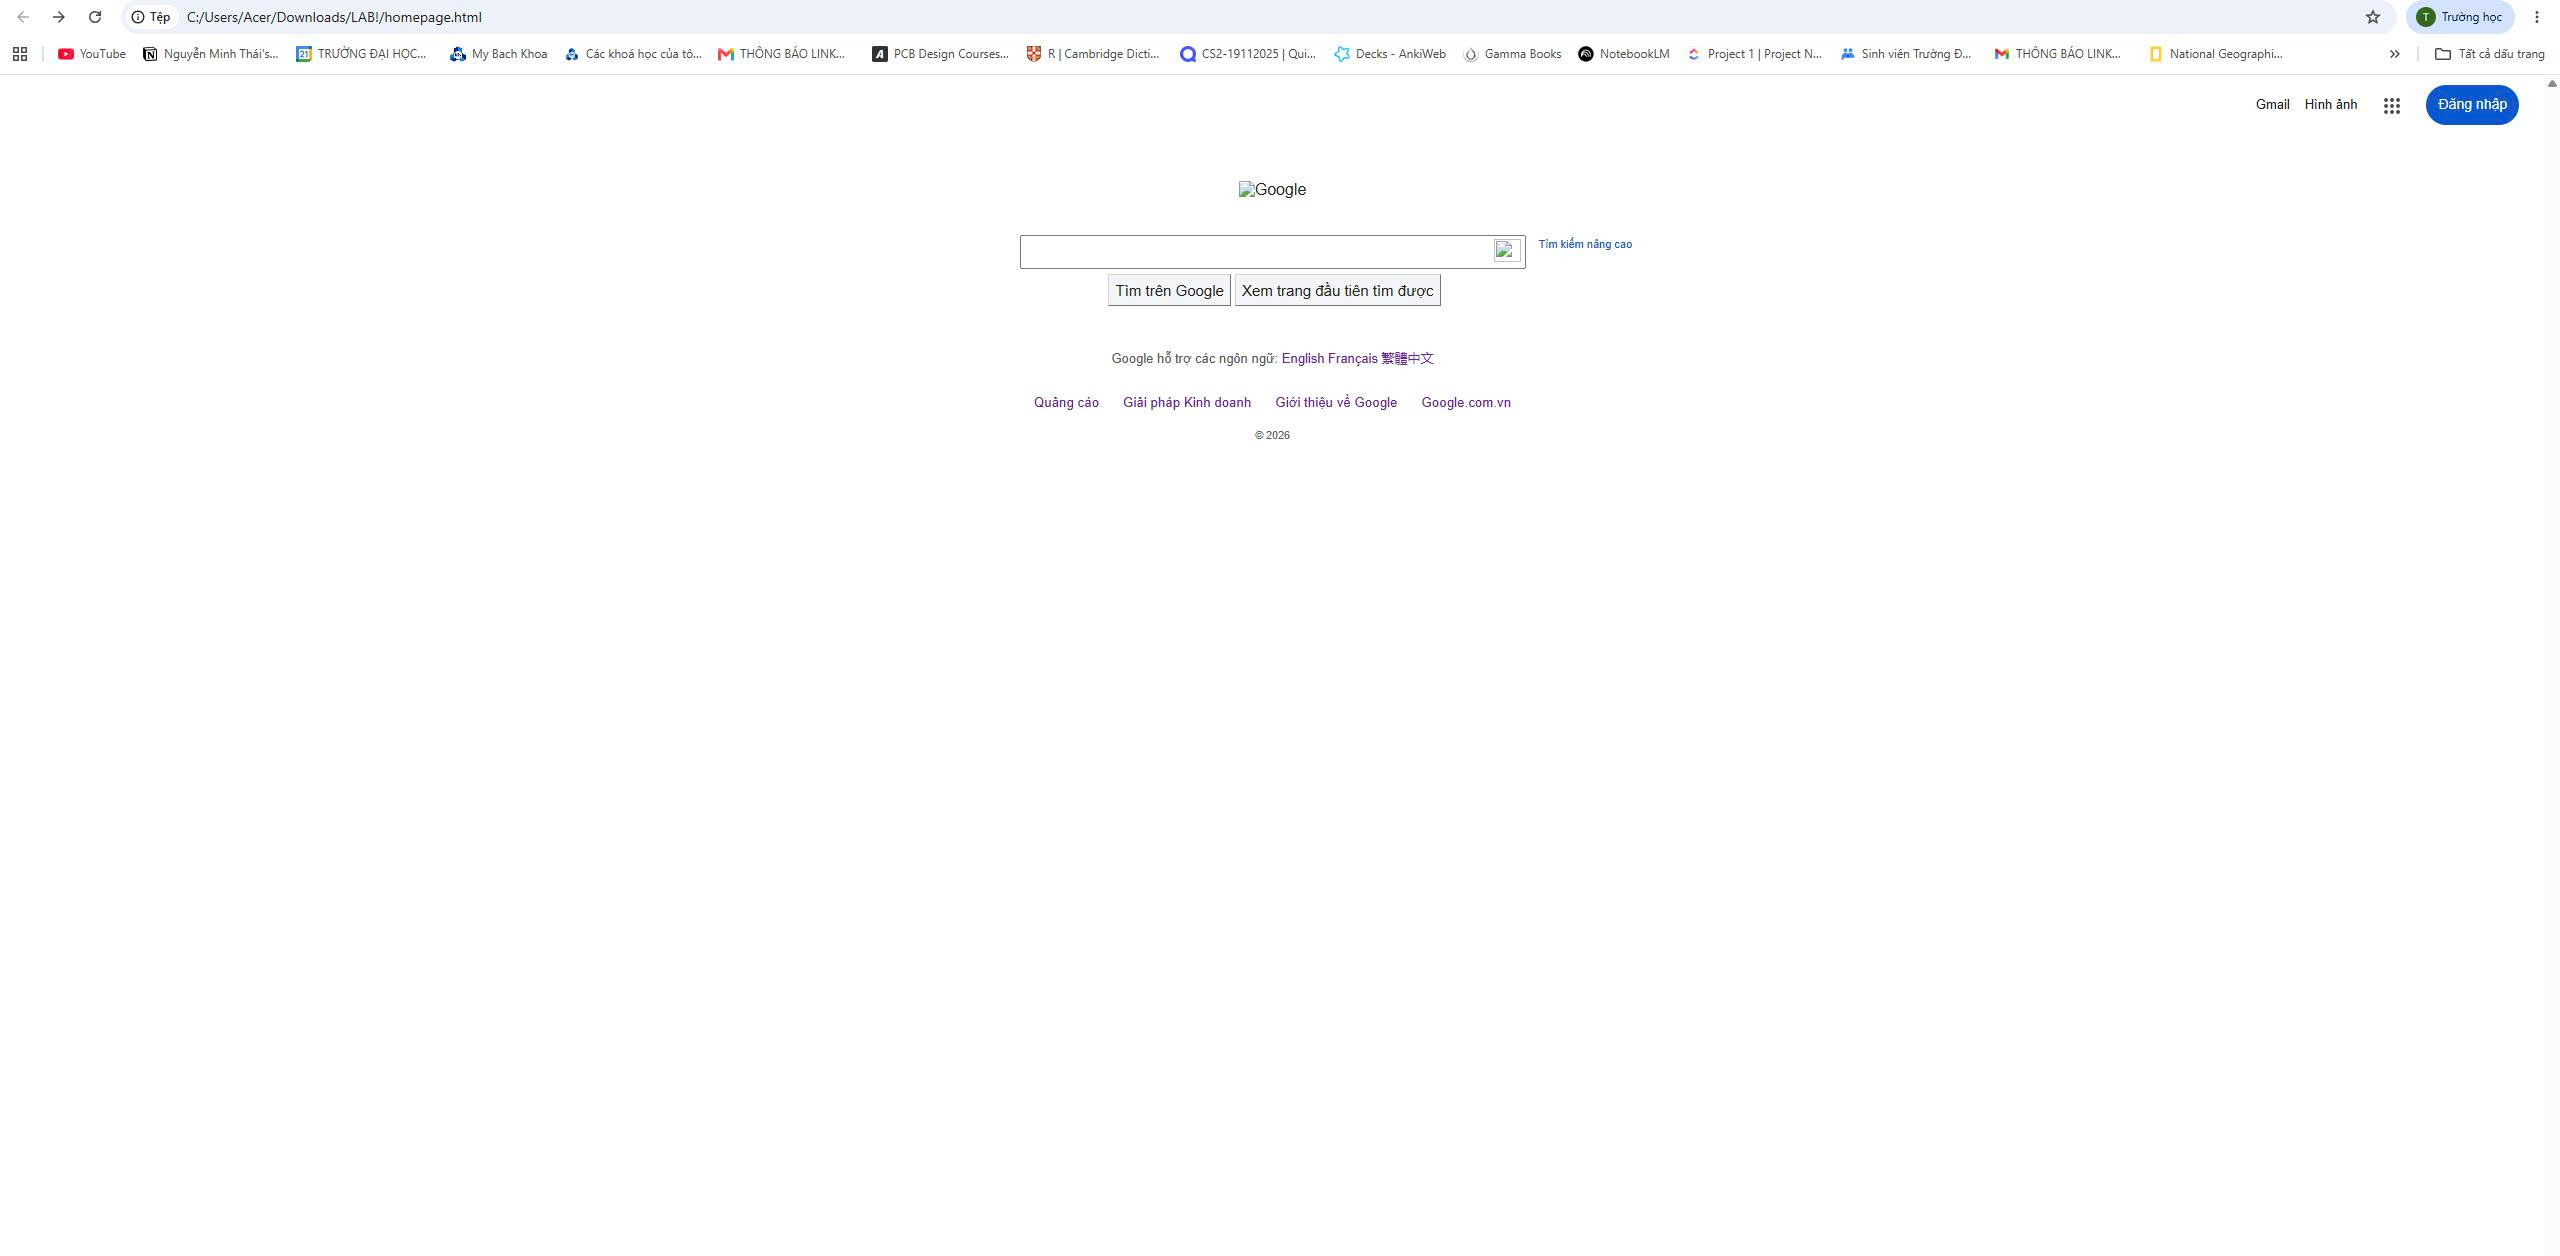
\includegraphics[width=0.7\textwidth]{images/homepage.jpg}
    
\end{center}   
\begin{center}
    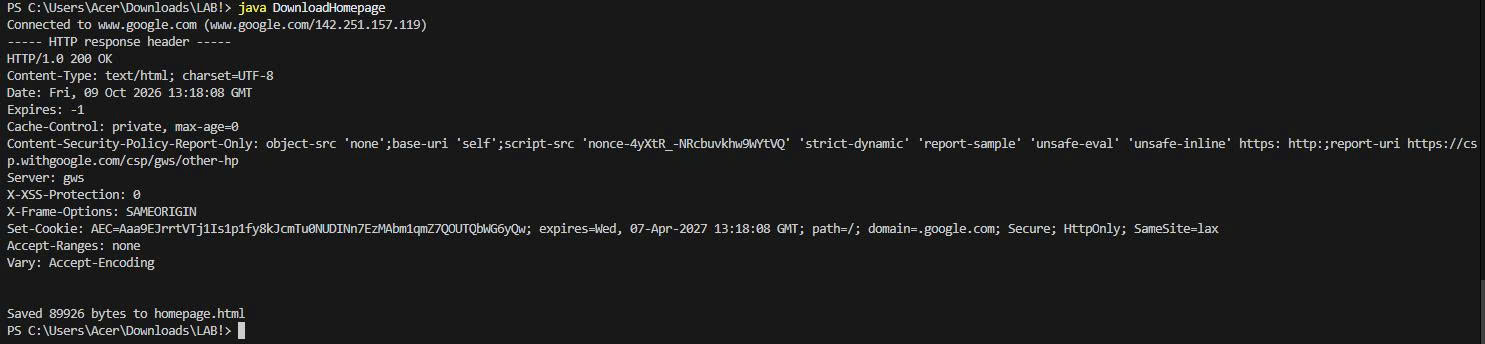
\includegraphics[width=0.9\textwidth]{images/homepage log.jpg}
\end{center}
{\footnotesize\textbf{Hình 1:} (Trái) Log phản hồi HTTP trên Terminal; (Phải) File \texttt{homepage.html} hiển thị trên trình duyệt.}
\vspace{0.4cm}
% \newpage

% ==================== 2. CHAT APPLICATION ====================
\subsection*{2. Develop a simple chat application using client-server model}

\begin{center}
\begin{tikzpicture}[
    scale=0.8, every node/.style={transform shape},
    steptext/.style={align=center, font=\sffamily\small},
    bluearr/.style={->, >=stealth, very thick, blue!80!black},
    redarr/.style={->, >=stealth, very thick, red!85!black}
]
    % --- PHÍA SERVER (Bên trái) ---
    \node[steptext] (s1) at (-2.0, 0.8) {
        create socket,\\
        port=x, for\\
        incoming request:\\
        {\color{red!85!black}\textbf{welcomeSocket =}}\\
        {\color{red!85!black}\textbf{ServerSocket()}}
    };

    \node[steptext] (s2) at (-2.0, -1.8) {
        wait for incoming\\
        connection request\\
        {\color{red!85!black}\textbf{connectionSocket =}}\\
        {\color{red!85!black}\textbf{welcomeSocket.accept()}}
    };

    \node[steptext] (s3) at (-2.0, -3.8) {
        read request from\\
        {\color{red!85!black}\textbf{connectionSocket}}
    };

    \node[steptext] (s4) at (-2.0, -5.2) {
        write reply to\\
        {\color{red!85!black}\textbf{connectionSocket}}
    };

    \node[steptext] (s5) at (-2.0, -6.5) {
        close\\
        {\color{red!85!black}\textbf{connectionSocket}}
    };

    % --- PHÍA CLIENT (Bên phải) ---
    \node[steptext] (c1) at (4.6, -1.8) {
        create socket,\\
        connect to hostid, port=x\\
        {\color{red!85!black}\textbf{clientSocket =}}\\
        {\color{red!85!black}\textbf{Socket()}}
    };

    \node[steptext] (c2) at (4.6, -3.5) {
        send request using\\
        {\color{red!85!black}\textbf{clientSocket}}
    };

    \node[steptext] (c3) at (4.6, -5.4) {
        read reply from\\
        {\color{red!85!black}\textbf{clientSocket}}
    };

    \node[steptext] (c4) at (4.6, -6.6) {
        close\\
        {\color{red!85!black}\textbf{clientSocket}}
    };

    % --- CÁC MŨI TÊN NỘI BỘ (XANH) ---
    \draw[bluearr] (s1) -- (s2) coordinate[midway] (arrow_mid);
    \draw[bluearr] (s2) -- (s3);
    \draw[bluearr] (s3) -- (s4);
    \draw[bluearr] (s4) -- (s5);

    % Mũi tên vòng lặp bên trái:
    % 1. Đi xuống (-7.1) kéo dài qua chữ một chút
    % 2. Đi ngang sang left (-5.2)
    % 3. Đi thẳng đứng lên đúng tọa độ y của (arrow_mid)
    % 4. Đi ngang sang right chỉ vuông góc vào thân mũi tên (arrow_mid)
    \draw[bluearr] (s5.south) -- (-2.0, -7.1) -- (-5.2, -7.1) |- (arrow_mid);

    \draw[bluearr] (c1) -- (c2);
    \draw[bluearr] (c2) -- (c3);
    \draw[bluearr] (c3) -- (c4);

    % --- GIAO TIẾP MẠNG (ĐỎ) ---
    % 1. TCP connection setup
    \draw[<->, >=stealth, dashed, line width=1.5pt, red!85!black] (0.1, -1.8) -- (2.3, -1.8)
        node[midway, above=1pt, font=\sffamily\bfseries\small, text=red!85!black]{TCP}
        node[midway, below=1pt, font=\sffamily\bfseries\small, text=red!85!black]{connection setup};

    % 2. Request từ Client sang Server
    \draw[redarr] (c2.west) -- (s3.east);

    % 3. Reply từ Server sang Client
    \draw[redarr] (s4.east) -- (c3.west);

    % --- KHUNG BAO NGOÀI ---
    \draw[draw=black!80, thick] (-5.6, -7.6) rectangle (6.8, 2.2);

\end{tikzpicture}
\end{center}

\begin{center}
\begin{tabularx}{\textwidth}{|X|X|}
\hline
\textbf{Server application} & \textbf{Client application} \\
\hline
Create a server socket & \\
\hline
Listen and wait for incoming connection request & Identify server IP and port \\
\hline
 & Create a TCP socket to the server \\
 & Establish a connection to the server \\
\hline
Accept the connection request & \\
\hline
Send/Receive data & Send/Receive data \\
\hline
 & Close connection \\
\hline
Close connection & \\
\hline
\end{tabularx}
\end{center}

\subsubsection*{Exercise 2: Design the user interface for the chat application}

\begin{solutionbox}[title=Báo cáo \& Bài làm: Exercise 2 -- Thiết kế Giao diện Ứng dụng Chat]
\textbf{1. Giao diện Server (\texttt{ChatServer.java}):}
\begin{itemize}
    \item Sử dụng Java Swing xây dựng cửa sổ điều khiển gồm: ô nhập Port lắng nghe (mặc định \texttt{9999}), nút bấm chuyển đổi trạng thái (\textit{Start / Stop}), và khung \texttt{JTextArea} có thanh cuộn hiển thị nhật ký kết nối và tin nhắn.
\end{itemize}

\textbf{2. Giao diện Client (\texttt{ChatClient.java}):}
\begin{itemize}
    \item \textbf{Form điều khiển chính (\texttt{Chat Client - Main}):} Ô nhập \texttt{Host} (\texttt{localhost}), \texttt{Port} (\texttt{9999}), \texttt{Name} (tên người dùng) và nút \textbf{"New connection"} để khởi tạo nhiều kết nối chat độc lập.
    \item \textbf{Cửa sổ chat riêng (\texttt{ChatWindow}):} Mỗi kết nối mở ra một cửa sổ riêng biệt với khung hiển thị lịch sử chat và ô nhập tin nhắn bên dưới, tự động gửi tin khi nhấn phím \texttt{Enter}.
\end{itemize}
\end{solutionbox}

\vspace{0.4cm}

% ==================== 3. MULTITHREAD IN JAVA ====================
\subsection*{3. Multithread in Java}
\noindent Create an application that has multiple threads running concurrently:
\begin{lstlisting}
class PrimeRun implements Runnable {
    long minPrime;
    PrimeRun ( long minPrime ) {
        this.minPrime = minPrime;
    }
    public void run() {
        // compute primes larger than minPrime
        . . .
    }
}
PrimeRun p = new PrimeRun(143);
new Thread(p).start();
\end{lstlisting}

\begin{solutionbox}[title=Báo cáo \& Bài làm: Lập trình Đa luồng (PrimeRun.java)]
\begin{itemize}
    \item \textbf{Nguyên lý cài đặt:} Lớp \texttt{PrimeRun} cài đặt \texttt{Runnable}, tính toán các số nguyên tố lớn hơn \texttt{minPrime} và kiểm tra cờ ngắt \texttt{!Thread.currentThread().isInterrupted()} trong vòng lặp.
    \item \textbf{Kiểm chứng chạy song song:} Trong hàm \texttt{main()}, hai luồng \texttt{T1} (mốc 143) và \texttt{T2} (mốc 1000) được khởi chạy đồng thời. Kết quả trên terminal cho thấy các số nguyên tố của \texttt{T1} và \texttt{T2} được in xen kẽ nhau, chứng minh CPU đã phân bổ thời gian thực thi song song (concurrency). Sau 20ms, lệnh \texttt{interrupt()} được gọi và cả hai luồng dừng lại an toàn.
\end{itemize}
\end{solutionbox}

\newpage 

\subsubsection*{Stop a thread:}
\noindent\textit{Try to use \texttt{Thread.interrupt()} as in the following code and see what happens.}
\begin{lstlisting}
public void stop() {
    running = false;
    this.interrupt();
}
public void run() {
    running = true;
    while (running) {
        Socket s = socket.accept();
        ...
    }
}
\end{lstlisting}

\begin{solutionbox}[title=Phân tích \& Giải thích: Cơ chế Dừng luồng khi bị tắc nghẽn ở accept()]
\textbf{1. Hiện tượng xảy ra khi gọi \texttt{stop()} dùng \texttt{this.interrupt()}:}
\begin{itemize}
    \item \textbf{Kết luận:} \textbf{Luồng Không thể dừng được Luồng tiếp tục bị kẹt và sống mãi mãi.}
\end{itemize}

\textbf{2. Bản chất nguyên nhân:}
\begin{enumerate}
    \item \textbf{Lời gọi bị chặn (Blocking I/O):} Phương thức \texttt{ServerSocket.accept()} là thao tác I/O đồng bộ bị chặn. Khi chưa có client nào kết nối, CPU treo luồng tại dòng này để đợi kết nối mạng.
    \item \textbf{Cơ chế \texttt{interrupt()} bị vô hiệu:} Trong Java I/O truyền thống, \texttt{accept()} không ném ra ngoại lệ \texttt{InterruptedException}. Gọi \texttt{this.interrupt()} chỉ bật cờ trạng thái ngắt, nhưng hàm \texttt{accept()} hoàn toàn phớt lờ cờ này.
    \item \textbf{Không bao giờ quay lại vòng lặp:} Do luồng đang bị kẹt cứng ở \texttt{accept()}, nó không thể thoát ra để quay lên đầu vòng lặp kiểm tra điều kiện \texttt{while (running)}. Vì vậy, gán \texttt{running = false} không có tác dụng.
\end{enumerate}

\textbf{3. Giải pháp chuẩn xác (\texttt{StopTest.java}):}
\begin{itemize}
    \item Để giải phóng luồng đang bị kẹt ở \texttt{accept()}, ta phải đóng socket từ luồng khác:
    $$\texttt{serverSocket.close();}$$
    \item Thao tác này ép buộc \texttt{accept()} giải phóng ngay lập tức và ném ra ngoại lệ:
    $$\texttt{java.net.SocketException: Socket closed}$$
    Khối \texttt{catch} sẽ bắt lấy ngoại lệ, luồng thoát khỏi vòng lặp và kết thúc an toàn.
\end{itemize}

\textbf{4. Kết quả thực nghiệm in ra từ Terminal:}
\begin{verbatim}
Testing running = false and t.interrupt()...
After interrupt, is thread alive? true
Testing serverSocket.close()...
accept() exited with: java.net.SocketException: Socket closed
Thread has stopped.
After close, is thread alive? false
\end{verbatim}


\end{solutionbox}

\newpage

\vspace{0.5cm}
\begin{center}
    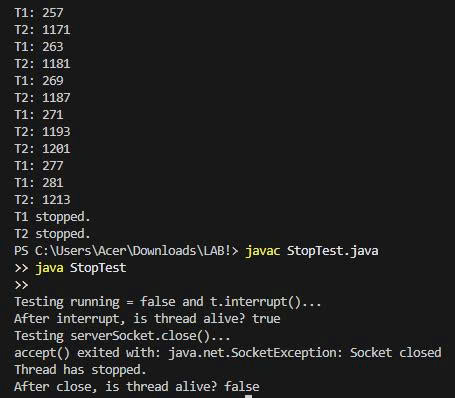
\includegraphics[width=0.40\textwidth]{images/PrimeRun and StopTest.jpg}\\[3pt]
    {\footnotesize \textbf{Hình 2:} Kết quả kiểm chứng đa luồng PrimeRun và cơ chế dừng thread StopTest.}
\end{center}



\subsubsection*{Multithread in Server Application:}
\begin{itemize}
    \item \textbf{Main window thread:} Chạy luồng giao diện Swing (Event Dispatch Thread).
    \item \textbf{Child thread (Listener):} Chạy vòng lặp \texttt{serverSocket.accept()} ngầm để đón kết nối mới mà không làm treo giao diện Server.
    \item \textbf{Grand-child thread (\texttt{ClientHandler}):} Tạo riêng cho từng Client kết nối để nhận dữ liệu và phát tin nhắn (broadcast).
\end{itemize}

\subsubsection*{Multithread in Client Application:}
\begin{itemize}
    \item \textbf{Main window thread:} Quản lý form nhập thông tin ban đầu.
    \item \textbf{Chat window thread:} Quản lý cửa sổ chat tương tác.
    \item \textbf{Grand-child thread (Reader):} Luồng chạy nền liên tục đọc \texttt{InputStream} từ server và cập nhật tin nhắn lên giao diện bằng \texttt{SwingUtilities.invokeLater()}.
\end{itemize}

\vspace{0.4cm}

\newpage

\subsubsection*{Exercise 3:}
\noindent\textit{Using multithread programming model to make the chat application can talk to many different users concurrently.}

\begin{solutionbox}[title=Báo cáo \& Bài làm: Exercise 3 -- Ứng dụng Chat Đa luồng Đồng thời]
\textbf{1. Kiến trúc Đa luồng \& Điểm nổi bật kỹ thuật:}
\begin{itemize}
    \item \textbf{Cơ chế Broadcast an toàn:} Server quản lý danh sách client bằng \texttt{CopyOnWriteArrayList<ClientHandler>}. Khi một client gửi tin nhắn, Server chuyển tiếp tin nhắn thời gian thực đến toàn bộ các client đang online.
    \item \textbf{Đóng kết nối sạch sẽ:} Khi người dùng tắt cửa sổ chat, socket tự đóng an toàn, Server tự động xóa client khỏi danh sách và thông báo cho mọi người (\texttt{*** [Name] left ***}).
\end{itemize}

\textbf{2. Kết quả Thử nghiệm Thực tế với 3 Thành viên Nhóm:}
\begin{itemize}
    \item \textbf{Kịch bản:} Khởi động \texttt{ChatServer} (Port 9999). Mở đồng thời 3 Client mang tên 3 thành viên: \textbf{Thái}, \textbf{Sơn}, và \textbf{Bảo}.
    \item \textbf{Kiểm chứng:} Khi các thành viên gửi tin nhắn (ví dụ: \textit{"Xin chào mọi người!"}, \textit{"Chào Thái nhé!"}, \textit{"Cùng bắt đầu nào"}), tin nhắn lập tức xuất hiện đồng bộ ở cả 3 cửa sổ và trên bảng Log của Server theo thời gian thực mà không gặp bất kỳ lỗi xung đột hay trễ luồng nào.
\end{itemize}


\end{solutionbox}

\vspace{0.2cm}
\begin{center}
    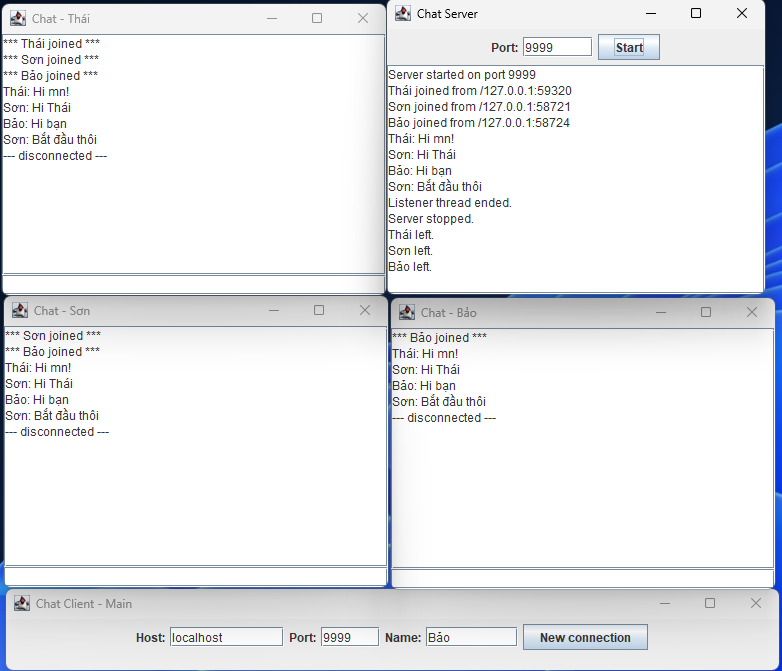
\includegraphics[width=0.8\textwidth]{images/Server Client.png}\\[3pt]
    {\footnotesize \textbf{Hình 3:} Giao diện ứng dụng Chat đa luồng thời gian thực với Server và 3 client.}
\end{center}


\vspace{0.5cm}



\end{document}
